% roomscan — SHORT version (<=10 pages) for the course report. Full version: main.tex + sections/.
% Translated from paper/draft/00–09 (Thai) on 2026-09-17; re-framed around R3 vs pretrained (ADR-014) on 2026-09-25.
% Numbers from experiments/results/*/table.md via scripts/paper_numbers.py -> numbers.tex.
% Build:  cd paper/latex && tectonic main_short.tex   or   pdflatex main_short && bibtex main_short && pdflatex x2
% Thai version (บทคัดย่อ): main_short_th.tex -> main_short_th.pdf (needs XeTeX/tectonic).
\documentclass[conference]{IEEEtran}
\IEEEoverridecommandlockouts

\usepackage[T1]{fontenc}
\usepackage[utf8]{inputenc}
\usepackage{amsmath,amssymb}
\usepackage{booktabs}
\usepackage{graphicx}
\usepackage{multirow}
\usepackage{adjustbox}
\usepackage{tabularx}
\usepackage{url}
\urlstyle{tt}
\usepackage{xcolor}
\usepackage{tikz}
\usetikzlibrary{positioning,arrows.meta}
\usepackage{pgfplots}   % Fig. 2 and 4 are drawn from ../figures/data/*.dat
\pgfplotsset{compat=1.18}
\usepackage{siunitx}
\usepackage[hidelinks]{hyperref}
\usepackage{cite}

\graphicspath{{../figures/}}
% Macros shared by main_short.tex (English) and main_short_th.tex (Thai). Load after siunitx.
\sisetup{detect-all,range-phrase=--,range-units=single,separate-uncertainty=true,multi-part-units=single}
\newcommand{\code}[1]{\texttt{#1}}
\newcommand{\fscore}{F@\SI{5}{cm}}
% The three fine-tunes, named teacher + number of training rooms (runs mono_ft_faro / mono_ft_lidar /
% mono_ft_lidar_all; ADR-014 calls them R1 / R2 / R3). \ftmain is the paper's main model.
\newcommand{\ftfaro}{\mbox{FT-Faro-10}}
\newcommand{\ftlidar}{\mbox{FT-LiDAR-10}}
\newcommand{\ftmain}{\mbox{FT-LiDAR-24}}
\hyphenation{LiDAR}   % never "Li-DAR"

\sloppy   % long code identifiers in prose: prefer loose lines over overfull boxes

\begin{document}

\title{Teaching Monocular Depth the Metre with the Phone's Own LiDAR:
Fine-Tuned vs.\ Pretrained Depth Anything~V2 for Room Reconstruction, Measured Against a Laser Scanner}

\author{\IEEEauthorblockN{1\textsuperscript{st} Panupong Duangdet}
\IEEEauthorblockA{\textit{dept. Master of Science Programme} \\
\textit{Software Engineering for Artificial Intelligence}\\
Bangkok, Thailand \\
email: dev.panupong@gmail.com\\
No.68130702310}
}

\maketitle

% generated by scripts/paper_numbers.py — do not edit

\newcommand{\rsGTCM}{2.1}
\newcommand{\rsGTSD}{0.5}
\newcommand{\rsGTF}{0.97}
\newcommand{\rsGTABSREL}{0.000}
\newcommand{\rsGTACC}{1.3}
\newcommand{\rsGTCOMP}{2.8}
\newcommand{\rsGTFtwo}{0.86}
\newcommand{\rsGTRtwo}{0.84}
\newcommand{\rsGTFfive}{0.97}
\newcommand{\rsGTRfive}{0.96}
\newcommand{\rsGTFten}{0.99}
\newcommand{\rsGTRten}{0.98}
\newcommand{\rsLIDARCM}{3.0}
\newcommand{\rsLIDARSD}{0.6}
\newcommand{\rsLIDARF}{0.93}
\newcommand{\rsLIDARABSREL}{0.018}
\newcommand{\rsLIDARACC}{2.2}
\newcommand{\rsLIDARCOMP}{3.9}
\newcommand{\rsLIDARFtwo}{0.54}
\newcommand{\rsLIDARRtwo}{0.52}
\newcommand{\rsLIDARFfive}{0.93}
\newcommand{\rsLIDARRfive}{0.91}
\newcommand{\rsLIDARFten}{0.98}
\newcommand{\rsLIDARRten}{0.97}
\newcommand{\rsORACLECM}{5.3}
\newcommand{\rsORACLESD}{1.3}
\newcommand{\rsORACLEF}{0.79}
\newcommand{\rsORACLEABSREL}{0.032}
\newcommand{\rsORACLEACC}{5.9}
\newcommand{\rsORACLECOMP}{4.7}
\newcommand{\rsORACLEFtwo}{0.46}
\newcommand{\rsORACLERtwo}{0.47}
\newcommand{\rsORACLEFfive}{0.79}
\newcommand{\rsORACLERfive}{0.82}
\newcommand{\rsORACLEFten}{0.90}
\newcommand{\rsORACLERten}{0.93}
\newcommand{\rsSPARSECM}{6.0}
\newcommand{\rsSPARSESD}{1.7}
\newcommand{\rsSPARSEF}{0.74}
\newcommand{\rsSPARSEABSREL}{0.036}
\newcommand{\rsSPARSEACC}{6.4}
\newcommand{\rsSPARSECOMP}{5.5}
\newcommand{\rsSPARSEFtwo}{0.38}
\newcommand{\rsSPARSERtwo}{0.39}
\newcommand{\rsSPARSEFfive}{0.74}
\newcommand{\rsSPARSERfive}{0.77}
\newcommand{\rsSPARSEFten}{0.88}
\newcommand{\rsSPARSERten}{0.91}
\newcommand{\rsSCENECM}{22.9}
\newcommand{\rsSCENESD}{2.1}
\newcommand{\rsSCENEF}{0.23}
\newcommand{\rsSCENEABSREL}{0.237}
\newcommand{\rsSCENEACC}{24.2}
\newcommand{\rsSCENECOMP}{21.6}
\newcommand{\rsSCENEFtwo}{0.08}
\newcommand{\rsSCENERtwo}{0.09}
\newcommand{\rsSCENEFfive}{0.23}
\newcommand{\rsSCENERfive}{0.27}
\newcommand{\rsSCENEFten}{0.41}
\newcommand{\rsSCENERten}{0.47}
\newcommand{\rsMETRICCM}{54.3}
\newcommand{\rsMETRICSD}{10.6}
\newcommand{\rsMETRICF}{0.03}
\newcommand{\rsMETRICABSREL}{0.382}
\newcommand{\rsMETRICACC}{70.3}
\newcommand{\rsMETRICCOMP}{38.3}
\newcommand{\rsMETRICFtwo}{0.01}
\newcommand{\rsMETRICRtwo}{0.01}
\newcommand{\rsMETRICFfive}{0.03}
\newcommand{\rsMETRICRfive}{0.04}
\newcommand{\rsMETRICFten}{0.06}
\newcommand{\rsMETRICRten}{0.10}
\newcommand{\rsGTa}{1.8}
\newcommand{\rsGTb}{1.2}
\newcommand{\rsGTc}{1.9}
\newcommand{\rsGTd}{2.8}
\newcommand{\rsGTe}{2.4}
\newcommand{\rsGTf}{2.3}
\newcommand{\rsLIDARa}{2.8}
\newcommand{\rsLIDARb}{2.4}
\newcommand{\rsLIDARc}{2.9}
\newcommand{\rsLIDARd}{4.1}
\newcommand{\rsLIDARe}{3.1}
\newcommand{\rsLIDARf}{3.0}
\newcommand{\rsORACLEa}{3.8}
\newcommand{\rsORACLEb}{6.2}
\newcommand{\rsORACLEc}{4.8}
\newcommand{\rsORACLEd}{7.5}
\newcommand{\rsORACLEe}{5.2}
\newcommand{\rsORACLEf}{4.5}
\newcommand{\rsSPARSEa}{4.5}
\newcommand{\rsSPARSEb}{6.1}
\newcommand{\rsSPARSEc}{5.5}
\newcommand{\rsSPARSEd}{9.1}
\newcommand{\rsSPARSEe}{5.9}
\newcommand{\rsSPARSEf}{4.6}
\newcommand{\rsSCENEa}{24.1}
\newcommand{\rsSCENEb}{26.0}
\newcommand{\rsSCENEc}{19.9}
\newcommand{\rsSCENEd}{23.2}
\newcommand{\rsSCENEe}{21.4}
\newcommand{\rsSCENEf}{23.1}
\newcommand{\rsMETRICa}{48.5}
\newcommand{\rsMETRICb}{61.6}
\newcommand{\rsMETRICc}{41.5}
\newcommand{\rsMETRICd}{48.9}
\newcommand{\rsMETRICe}{54.1}
\newcommand{\rsMETRICf}{71.0}
\newcommand{\rsFTFAROa}{10.8}
\newcommand{\rsFTFAROb}{13.8}
\newcommand{\rsFTFAROc}{17.6}
\newcommand{\rsFTFAROd}{21.1}
\newcommand{\rsFTFAROe}{12.4}
\newcommand{\rsFTFAROf}{11.9}
\newcommand{\rsFTLIDARa}{13.9}
\newcommand{\rsFTLIDARb}{19.0}
\newcommand{\rsFTLIDARc}{12.8}
\newcommand{\rsFTLIDARd}{12.5}
\newcommand{\rsFTLIDARe}{16.6}
\newcommand{\rsFTLIDARf}{24.6}
\newcommand{\rsFTLIDARALLa}{12.8}
\newcommand{\rsFTLIDARALLb}{16.7}
\newcommand{\rsFTLIDARALLc}{17.3}
\newcommand{\rsFTLIDARALLd}{12.2}
\newcommand{\rsFTLIDARALLe}{12.4}
\newcommand{\rsFTLIDARALLf}{22.5}
\newcommand{\rsSPARSEGAP}{0.6}
\newcommand{\rsSPARSEGAPLIDAR}{2.9}
\newcommand{\rsSPARSEVSSCENE}{3.8}
\newcommand{\rsLIDARGAPGTCM}{0.98}
\newcommand{\rsLIDARGAPGTSD}{0.25}
\newcommand{\rsORACLEGAPLIDARCM}{2.29}
\newcommand{\rsORACLEGAPLIDARSD}{1.11}
\newcommand{\rsCONFONECM}{3.07}
\newcommand{\rsCONFONEF}{0.93}
\newcommand{\rsCONFONEACC}{2.17}
\newcommand{\rsCONFONECOMP}{3.98}
\newcommand{\rsCONFTWOCM}{3.66}
\newcommand{\rsCONFTWOF}{0.93}
\newcommand{\rsCONFTWOACC}{2.08}
\newcommand{\rsCONFTWOCOMP}{5.23}
\newcommand{\rsWZOTCM}{3.07}
\newcommand{\rsWZOTF}{0.93}
\newcommand{\rsWZOTACC}{2.17}
\newcommand{\rsWZOTCOMP}{3.98}
\newcommand{\rsWOTFCM}{3.04}
\newcommand{\rsWOTFF}{0.93}
\newcommand{\rsWOTFACC}{2.23}
\newcommand{\rsWOTFCOMP}{3.85}
\newcommand{\rsFTFAROCM}{14.6}
\newcommand{\rsFTFAROSD}{4.0}
\newcommand{\rsFTFAROF}{0.31}
\newcommand{\rsFTFAROABSREL}{0.136}
\newcommand{\rsFTFARODELTAONE}{0.780}
\newcommand{\rsFTFARORtwo}{0.12}
\newcommand{\rsFTFARORfive}{0.34}
\newcommand{\rsFTFARORten}{0.57}
\newcommand{\rsFTLIDARCM}{16.6}
\newcommand{\rsFTLIDARSD}{4.7}
\newcommand{\rsFTLIDARF}{0.23}
\newcommand{\rsFTLIDARABSREL}{0.136}
\newcommand{\rsFTLIDARDELTAONE}{0.848}
\newcommand{\rsFTLIDARRtwo}{0.09}
\newcommand{\rsFTLIDARRfive}{0.26}
\newcommand{\rsFTLIDARRten}{0.49}
\newcommand{\rsFTLIDARALLCM}{15.7}
\newcommand{\rsFTLIDARALLSD}{4.0}
\newcommand{\rsFTLIDARALLF}{0.24}
\newcommand{\rsFTLIDARALLABSREL}{0.134}
\newcommand{\rsFTLIDARALLDELTAONE}{0.812}
\newcommand{\rsFTLIDARALLRtwo}{0.09}
\newcommand{\rsFTLIDARALLRfive}{0.28}
\newcommand{\rsFTLIDARALLRten}{0.51}
\newcommand{\rsFTTEACHERRATIO}{1.13}
\newcommand{\rsFTGAIN}{3.3}
\newcommand{\rsFTGAPORACLE}{11.2}
\newcommand{\rsDALARGECM}{6.45}
\newcommand{\rsDALARGESD}{2.42}
\newcommand{\rsDALARGEF}{0.74}
\newcommand{\rsDALARGEABSREL}{0.040}
\newcommand{\rsDALARGEDELTAONE}{0.979}
\newcommand{\rsDALARGESCAN}{355}
\newcommand{\rsDASMALLCM}{9.22}
\newcommand{\rsDASMALLSD}{3.48}
\newcommand{\rsDASMALLF}{0.64}
\newcommand{\rsDASMALLABSREL}{0.054}
\newcommand{\rsDASMALLDELTAONE}{0.964}
\newcommand{\rsDASMALLSCAN}{56}
\newcommand{\rsMIDASCM}{14.95}
\newcommand{\rsMIDASSD}{1.87}
\newcommand{\rsMIDASF}{0.35}
\newcommand{\rsMIDASABSREL}{0.110}
\newcommand{\rsMIDASDELTAONE}{0.873}
\newcommand{\rsMIDASSCAN}{18}
\newcommand{\rsSTRGTONECM}{2.1}
\newcommand{\rsSTRGTONEACC}{1.3}
\newcommand{\rsSTRGTONECOMP}{2.8}
\newcommand{\rsSTRGTONEF}{0.97}
\newcommand{\rsSTRGTONEABSREL}{0.000}
\newcommand{\rsSTRGTONEN}{391}
\newcommand{\rsSTRGTONESCAN}{2}
\newcommand{\rsSTRGTFIVECM}{4.4}
\newcommand{\rsSTRGTFIVEACC}{1.2}
\newcommand{\rsSTRGTFIVECOMP}{7.5}
\newcommand{\rsSTRGTFIVEF}{0.91}
\newcommand{\rsSTRGTFIVEABSREL}{0.000}
\newcommand{\rsSTRGTFIVEN}{78}
\newcommand{\rsSTRGTFIVESCAN}{1}
\newcommand{\rsSTRGTTENCM}{8.9}
\newcommand{\rsSTRGTTENACC}{1.2}
\newcommand{\rsSTRGTTENCOMP}{16.6}
\newcommand{\rsSTRGTTENF}{0.83}
\newcommand{\rsSTRGTTENABSREL}{0.000}
\newcommand{\rsSTRGTTENN}{40}
\newcommand{\rsSTRGTTENSCAN}{1}
\newcommand{\rsSTRGTTWENTYCM}{16.8}
\newcommand{\rsSTRGTTWENTYACC}{1.2}
\newcommand{\rsSTRGTTWENTYCOMP}{32.3}
\newcommand{\rsSTRGTTWENTYF}{0.68}
\newcommand{\rsSTRGTTWENTYABSREL}{0.000}
\newcommand{\rsSTRGTTWENTYN}{20}
\newcommand{\rsSTRGTTWENTYSCAN}{1}
\newcommand{\rsSTRORACLEONECM}{6.5}
\newcommand{\rsSTRORACLEONEACC}{7.1}
\newcommand{\rsSTRORACLEONECOMP}{5.8}
\newcommand{\rsSTRORACLEONEF}{0.74}
\newcommand{\rsSTRORACLEONEABSREL}{0.040}
\newcommand{\rsSTRORACLEONEN}{391}
\newcommand{\rsSTRORACLEONESCAN}{358}
\newcommand{\rsSTRORACLEFIVECM}{8.2}
\newcommand{\rsSTRORACLEFIVEACC}{5.6}
\newcommand{\rsSTRORACLEFIVECOMP}{10.9}
\newcommand{\rsSTRORACLEFIVEF}{0.72}
\newcommand{\rsSTRORACLEFIVEABSREL}{0.040}
\newcommand{\rsSTRORACLEFIVEN}{78}
\newcommand{\rsSTRORACLEFIVESCAN}{72}
\newcommand{\rsSTRORACLETENCM}{12.7}
\newcommand{\rsSTRORACLETENACC}{5.0}
\newcommand{\rsSTRORACLETENCOMP}{20.3}
\newcommand{\rsSTRORACLETENF}{0.65}
\newcommand{\rsSTRORACLETENABSREL}{0.041}
\newcommand{\rsSTRORACLETENN}{40}
\newcommand{\rsSTRORACLETENSCAN}{36}
\newcommand{\rsSTRORACLETWENTYCM}{20.9}
\newcommand{\rsSTRORACLETWENTYACC}{5.1}
\newcommand{\rsSTRORACLETWENTYCOMP}{36.7}
\newcommand{\rsSTRORACLETWENTYF}{0.52}
\newcommand{\rsSTRORACLETWENTYABSREL}{0.040}
\newcommand{\rsSTRORACLETWENTYN}{20}
\newcommand{\rsSTRORACLETWENTYSCAN}{19}
\newcommand{\rsSTRSCENEONECM}{22.7}
\newcommand{\rsSTRSCENEONEACC}{23.8}
\newcommand{\rsSTRSCENEONECOMP}{21.7}
\newcommand{\rsSTRSCENEONEF}{0.22}
\newcommand{\rsSTRSCENEONEABSREL}{0.240}
\newcommand{\rsSTRSCENEONEN}{391}
\newcommand{\rsSTRSCENEONESCAN}{346}
\newcommand{\rsSTRSCENEFIVECM}{22.7}
\newcommand{\rsSTRSCENEFIVEACC}{20.2}
\newcommand{\rsSTRSCENEFIVECOMP}{25.2}
\newcommand{\rsSTRSCENEFIVEF}{0.23}
\newcommand{\rsSTRSCENEFIVEABSREL}{0.236}
\newcommand{\rsSTRSCENEFIVEN}{78}
\newcommand{\rsSTRSCENEFIVESCAN}{71}
\newcommand{\rsSTRSCENETENCM}{25.0}
\newcommand{\rsSTRSCENETENACC}{18.9}
\newcommand{\rsSTRSCENETENCOMP}{31.0}
\newcommand{\rsSTRSCENETENF}{0.20}
\newcommand{\rsSTRSCENETENABSREL}{0.247}
\newcommand{\rsSTRSCENETENN}{40}
\newcommand{\rsSTRSCENETENSCAN}{36}
\newcommand{\rsSTRSCENETWENTYCM}{34.5}
\newcommand{\rsSTRSCENETWENTYACC}{21.4}
\newcommand{\rsSTRSCENETWENTYCOMP}{47.6}
\newcommand{\rsSTRSCENETWENTYF}{0.14}
\newcommand{\rsSTRSCENETWENTYABSREL}{0.268}
\newcommand{\rsSTRSCENETWENTYN}{20}
\newcommand{\rsSTRSCENETWENTYSCAN}{19}

\begin{abstract}
Devices without LiDAR can reconstruct a room from monocular depth, but an off-the-shelf ``metric'' model such as Depth
Anything~V2 Metric-Indoor, trained on synthetic images, misplaces a real room by \SI{\rsMETRICCM}{cm} inside a
reconstruction pipeline. We ask whether fine-tuning it with depth from the phone's own LiDAR---no laser scanner
involved---makes it better than its pretrained self when measured against the Faro laser scanner that ARKitScenes ships.
We fine-tune only the DPT head on 24 ARKitScenes rooms with iPad LiDAR labels (R3) and compare it with the pretrained
checkpoint through one depth $\rightarrow$ TSDF $\rightarrow$ mesh pipeline in which the depth source is the single
variable, on rooms never used for training: six rooms with a Faro reference mesh (3D and 2D) and \rsVN{} further rooms
(2D, \rsVFRAMES{} frames). R3 lowers Chamfer from \SI{\rsMETRICCM}{cm} to \SI{\rsFTLIDARALLCM}{cm} ($\rsMAINGAIN\times$,
better in every room) and per-frame AbsRel from \rsVMETRICABSREL{} to \rsVFTALLABSREL{} on the \rsVN{} unseen rooms
(better in \rsVWINS/\rsVN), with no calibration or sensor at run time. A laser teacher (\SI{\rsFTFAROCM}{cm}) is not
measurably better. For context, the same pipeline gives \SI{\rsLIDARCM}{cm} with iPad LiDAR and \SI{\rsSPARSECM}{cm} with
a monocular model scaled per frame on $\sim$200 sparse metric points. Per-frame analysis shows that R3's remaining error
is a scale that swings with the content of each view, which fine-tuning de-biases but does not remove: the rooms are a
large step toward, but not yet at, overview accuracy. Code, configs, per-run metrics and checkpoints are released.
\end{abstract}


\begin{IEEEkeywords}
monocular depth estimation, transfer learning, metric depth, LiDAR supervision, TSDF fusion, 3D room reconstruction, ARKitScenes
\end{IEEEkeywords}

\section{Introduction and Business Motivation}

Scanning a room into a 3D model is already a consumer feature on iPhone~Pro and iPad~Pro (Apple RoomPlan, Polycam),
all relying on the \emph{LiDAR sensor} for metric depth. Devices with LiDAR are, however, a minority: non-Pro iPhones
and almost every Android phone have none. Their alternative is \emph{monocular depth estimation}, which advanced
rapidly between 2020 and 2024 (MiDaS, Depth Anything). A product team must know \textbf{by how many centimetres the
room is wrong if LiDAR is replaced by a monocular model, and which use cases that still serves}---a question per-image
benchmark metrics (AbsRel, $\delta_1$) do not answer, and end-to-end reconstruction systems (Atlas, NeuralRecon,
SimpleRecon) cannot answer because they design the whole pipeline around their own model.

Some recent models claim to output metres directly (DA-v2 Metric-Indoor, ZoeDepth, Depth Pro), but they are trained
on data that is not a phone's camera---DA-v2 Metric-Indoor on rendered Hypersim images---and inside a real
reconstruction pipeline the room comes out \SI{\rsMETRICCM}{cm} wrong (\S\ref{sec:exp1}). The direct remedy is
\emph{transfer learning} on target-domain depth. The question is where the labels come from: a \$20k laser scanner,
or the \emph{LiDAR already inside Pro phones}, which an app maker can collect at scale. If the latter works, devices
with LiDAR can teach those without it.

\textbf{Research question.} Is DA-v2 Metric-Indoor fine-tuned with iPad LiDAR depth (no laser scanner at training
time) better than the same model pretrained, measured against the Faro laser scanner---as a room mesh and as per-frame
depth---on rooms never used for training? \textbf{Supporting questions:} (a) is a laser teacher better than a
phone-LiDAR teacher; (b) where does the fine-tuned model stand relative to a sensor at run time; (c) where does the
remaining error come from?

\textbf{Approach.} We build a classical pipeline (per-frame depth $\rightarrow$ scale alignment $\rightarrow$ TSDF
fusion $\rightarrow$ mesh) in which \textbf{the depth source is the single swappable variable}, so ``pretrained'' and
``fine-tuned'' are two rows differing only in a checkpoint, and every other depth source (Faro laser, ARKit LiDAR,
relative monocular models with different scale strategies) is priced through the same pipeline as context.

\textbf{Contributions.}
\begin{enumerate}
\item A measured answer to whether fine-tuning a metric monocular model on a phone's own LiDAR helps, against a laser
scanner on held-out rooms in 3D (6 rooms) and 2D (6 $+$ \rsVN{} rooms), with checkpoints and room split released.
\item A teacher ablation (Faro vs.\ LiDAR, 10 vs.\ 24 rooms) and an intrinsics-conditioned baseline (Depth Pro).
\item An open-source pipeline in which \code{DepthSource} and \code{ScaleAligner} are interfaces switched from config,
so every table is ``one loop, one variable.''
\item ``Centimetres on the wall'' for laser / LiDAR / monocular $\times$ scale strategy, and an analysis showing that
monocular error comes from per-view scale, not temporal drift---explaining why fine-tuning helps and why it is not
enough.
\end{enumerate}

\textbf{Not claimed.} We do not compare against Atlas / NeuralRecon / SimpleRecon; we do not claim fine-tuning makes
LiDAR unnecessary (\ftmain{} at \SI{\rsFTLIDARALLCM}{cm} remains far from LiDAR at \SI{\rsLIDARCM}{cm}); and since training and
testing use the same iPad camera, transfer to other phone cameras is not measured.

\section{Related Work}\label{sec:related}

\textbf{Relative monocular depth.} MiDaS~\cite{midas} trains across datasets with a scale- and shift-invariant loss,
so its output is disparity up to an affine transform: two constants $(s,t)$ per image are needed for metres. Depth
Anything~\cite{da1} and V2~\cite{da2} scale this idea with large unlabelled corpora. We treat $(s,t)$ as an
experimental variable (the \code{ScaleAligner}) rather than hiding it in the model.

\textbf{Metric monocular depth.} ZoeDepth~\cite{zoedepth} and the metric DA-v2 variants (fine-tuned on Hypersim /
Virtual KITTI) output metres directly. Metric3D~\cite{metric3d}, UniDepth~\cite{unidepth} and Depth Pro~\cite{depthpro}
instead condition on, or estimate, camera intrinsics. These works report per-image metrics on NYUv2/KITTI; we show
that on real room video the per-frame scale of a metric model still swings widely within one scan---invisible to
per-image metrics, obvious once frames are fused. The closest work in data is Prompt Depth Anything~\cite{promptda},
which feeds iPhone LiDAR to the network \emph{at run time} on ARKitScenes; we instead use LiDAR only as a
\emph{training} teacher, so the deployed model needs no depth sensor.

\textbf{Depth fusion and learned reconstruction.} TSDF fusion~\cite{curless96,kinectfusion} neither knows nor cares
where metric, posed depth comes from, making it a fair fixed stage for every source; we use Open3D~\cite{open3d}.
Atlas~\cite{atlas}, NeuralRecon~\cite{neuralrecon} and SimpleRecon~\cite{simplerecon} learn depth or TSDF from
multiple images and are strong ScanNet baselines, but do not answer what room a per-image model plus the device's VIO
pose yields, so we do not compare against them. Scale recovery from sparse tracked points follows
CNN-SLAM~\cite{cnnslam} and MonoSDF~\cite{monosdf}; our \code{sparse\_points} aligner belongs to this line.

\textbf{Mobile LiDAR and products.} ARKitScenes~\cite{arkitscenes} is the first dataset releasing both iPad LiDAR
depth and Faro laser depth for the same rooms. RoomPlan~\cite{roomplan} and similar apps require LiDAR, and no public
report states how many centimetres they deviate from a laser scanner.

\section{Methodology}\label{sec:method}
% Thai version: 03_methodology_th.tex (main_short_th.tex); keep the two in step.
% Replaces the former 03_system_design.tex + 04_experimental_setup.tex of the short version.

The study compares depth sources inside one fixed reconstruction pipeline (Fig.~\ref{fig:pipeline}). For every room
and every depth source it (1)~reads the colour frames and camera poses, (2)~obtains a depth map for every frame from
the source, (3)~converts that depth to metres if the source does not give metres, (4)~fuses the frames into a room
mesh, and (5)~measures the per-frame depth and the mesh against the Faro reference. Only steps (2) and (3) change
between the rows of a result table; each is chosen by one entry of a configuration file, and every later step runs the
same code with the same settings. The fine-tuned models enter at step~(2) as ordinary depth sources. This section
describes the data, each step, the fine-tuning, the metrics and statistics, and the experiments.

\begin{figure*}[t]
\centering
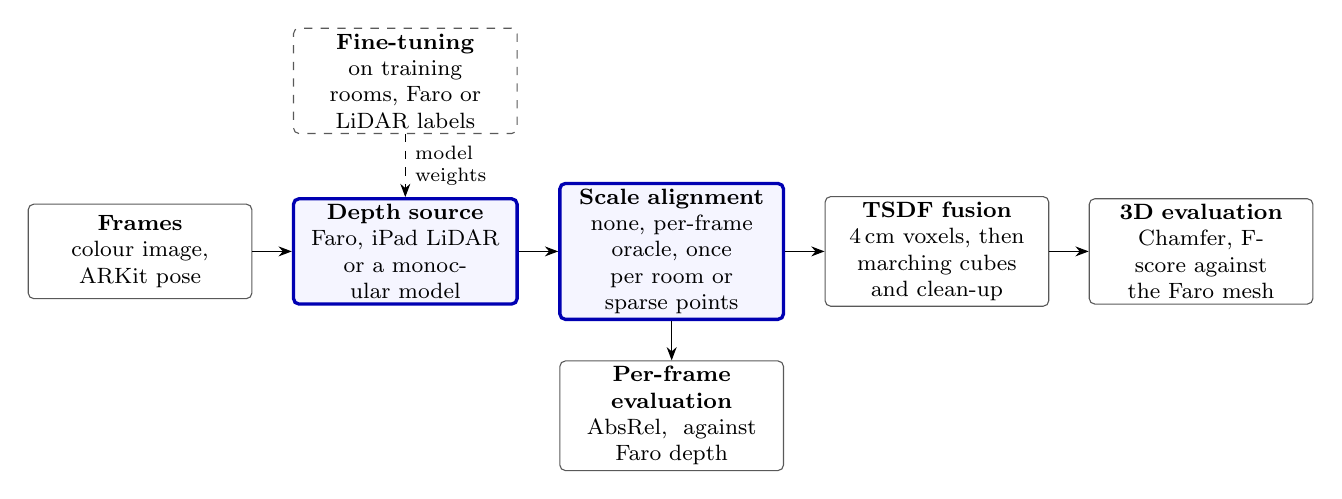
\begin{tikzpicture}[font=\footnotesize, >=Stealth, node distance=5mm,
  box/.style={draw=black!65, rounded corners=2pt, align=center, text width=27mm, minimum height=12mm, inner sep=2pt},
  swap/.style={box, draw=blue!70!black, very thick, fill=blue!4},
  side/.style={box, dashed}]
\node[box]  (in)   {\textbf{Frames}\\colour image, ARKit pose};
\node[swap, right=of in]  (src)  {\textbf{Depth source}\\Faro, iPad LiDAR or a monocular model};
\node[swap, right=of src] (aln)  {\textbf{Scale alignment}\\none, per-frame oracle, once per room or sparse points};
\node[box, right=of aln]  (fus)  {\textbf{TSDF fusion}\\\SI{4}{cm} voxels, then marching cubes and clean-up};
\node[box, right=of fus]  (ev3)  {\textbf{3D evaluation}\\Chamfer, F-score against the Faro mesh};
\node[side, above=8mm of src] (ft)   {\textbf{Fine-tuning}\\on training rooms, Faro or LiDAR labels};
\node[box, below=of aln]  (ev2)  {\textbf{Per-frame evaluation}\\AbsRel, \wone{} against Faro depth};
\draw[->] (in) -- (src); \draw[->] (src) -- (aln); \draw[->] (aln) -- (fus); \draw[->] (fus) -- (ev3);
\draw[->, dashed] (ft) -- node[right, align=left, font=\scriptsize] {model\\weights} (src);
\draw[->] (aln) -- (ev2);
\end{tikzpicture}
\caption{Pipeline. The two highlighted steps are the only ones that change between the rows of a result table, each
by one configuration entry; every step after them is fixed. Fine-tuning (dashed) happens once, beforehand, and only
supplies the weights of a monocular model.}
\label{fig:pipeline}
\end{figure*}

\subsection{Data, rooms and reference}\label{sec:data}
ARKitScenes~\cite{arkitscenes} provides, for the same room, the colour video of an iPad~Pro ($640\times480$ pixels),
the depth of its LiDAR as produced by ARKit ($256\times192$ pixels, with a confidence of low, medium or high for every
pixel), the camera pose of every frame from ARKit's visual-inertial odometry, and depth from a Faro laser
scanner~\cite{faro} registered to those poses ($1920\times1440$ pixels, about four frames per second).
\textbf{The ground truth is this Faro depth as distributed.} For per-frame evaluation it is resampled to
$256\times192$ by taking the nearest pixel, so every reference value is a measured one. For 3D evaluation, since no
laser mesh is distributed, we fuse the Faro depth of every frame at \SI{1}{cm} voxels, once per room, into a
reference mesh with the fusion of Section~\ref{sec:fusion}. Because this reference and every depth source use the same
poses, pose error is excluded and every difference between rows is due to the depth source. iPad LiDAR is never used
as ground truth.

\begin{table}[t]
\centering\small
\caption{Test rooms, evaluated in 3D and per frame. Frames: Faro frames on which every row is evaluated.}
\label{tab:scenes}
\begin{adjustbox}{max width=\columnwidth}
\begin{tabular}{@{}llrr@{}}
\toprule
Scan ID & Room & Extent (m) & Frames \\
\midrule
42444474 & kitchen/dining with glass (development room) & $9.9\times5.1\times4.2$ & 236 \\
47333774 & standard bedroom & $5.1\times4.9\times3.3$ & 375 \\
47115299 & large living room & $8.1\times6.1\times2.5$ & 324 \\
42897743 & bathroom (mirror, tiles) & $8.0\times3.4\times3.6$ & 448 \\
47429736 & bedroom with closets & $6.6\times6.4\times2.7$ & 504 \\
45261556 & kitchen (glossy cabinets) & $7.1\times6.1\times2.4$ & 465 \\
\bottomrule
\end{tabular}
\end{adjustbox}
\end{table}

The six test rooms (Table~\ref{tab:scenes}) span a standard bedroom, large rooms and rooms with mirrors or glossy
surfaces. Room 42444474 was used while the pipeline was developed, so its numbers are not held out; the per-room
results let the reader check every conclusion on the other five. The rooms for fine-tuning were drawn at random
(seed~0) from ARKitScenes scans of 60 to \SI{120}{s}, excluding every visit of a test room, a visit being the capture
session of one home, whose videos show the same rooms: 10 training rooms with both Faro and LiDAR depth, 14 more with
LiDAR only, and 3 rooms of the dataset's Validation fold for choosing the checkpoint. Exp.~7 adds \rsVN{} further
Validation-fold rooms, one video per visit, drawn with seed~0 and excluding every visit of the training,
checkpoint-selection and test rooms. They decided nothing and are evaluated per frame only, on every second Faro frame
(\rsVFRAMES{} frames in total).

\subsection{Depth sources}\label{sec:sources}
Four kinds of depth source are compared. (1)~The Faro depth itself shows what the pipeline loses when depth is perfect:
at \SI{4}{cm} voxels it still differs from the \SI{1}{cm} reference, and that difference is the pipeline's own
discretisation loss. (2)~The iPad LiDAR depth as recorded by ARKit is what a Pro device uses today. (3)~Relative
monocular models need the scale alignment of Section~\ref{sec:align}: DA-v2 Large in the main experiments, and DA-v2
Small and MiDaS small~\cite{midas} when model size is varied. (4)~Metric monocular models are used with no alignment:
DA-v2 Metric-Indoor Large, pretrained; its three fine-tunes (Section~\ref{sec:ftsetup}); and Depth Pro~\cite{depthpro},
given the camera's true focal length of 533 pixels, its most favourable setting. Its implementation was checked on
a synthetic room with exact depth; on five frames of room 47115299 it was also run with its own estimate of the field
of view and scored after removing the scale of each frame. ARKitScenes stores the frames of an
iPad held upright rotated by a quarter turn, so every monocular model receives the frame rotated upright and its output
is rotated back. Every source is resampled by nearest pixel to the LiDAR resolution of $256\times192$, so that all
sources are fused and scored on the same grid.

\subsection{Scale alignment}\label{sec:align}
A relative model gives inverse depth that is known only up to a scale and an offset per image
(Section~\ref{sec:related}). Alignment finds the scale and offset that make the model's inverse depth best match a set
of reference depths, also inverted, and converts the result back to depth. Fitting in inverse depth rather than in
depth follows how these models are trained; on the development room it reduced the Chamfer distance of the per-frame
oracle from 15.2 to \SI{5.4}{cm}. The fit is by least squares, repeated three times, each time leaving out the
20\,\% of pixels with the largest residuals, because depth edges produce a few very large residuals that would
otherwise pull the fit. The four alignments differ only in the reference depths they fit against
(Table~\ref{tab:aligners}); a metric source is always used with no alignment, and the pipeline refuses to run
otherwise.

\begin{table}[t]
\centering\small
\caption{Scale alignments. Every alignment other than ``none'' fits one scale and one offset in inverse depth by
trimmed least squares.}
\label{tab:aligners}
\begin{tabularx}{\columnwidth}{@{}l>{\raggedright\arraybackslash}X@{}}
\toprule
Alignment & Fitted on, and what the row shows \\
\midrule
none & nothing; used for Faro, LiDAR and metric models \\
per-frame oracle & the frame's own Faro depth; the best the model's shape allows (not usable in a product) \\
once per room & Faro depth of 10 frames spread evenly over the scan, fitted once and kept for every frame; an upper
bound of a one-off calibration \\
sparse points & 200 metric points per frame, standing for the feature points of VIO (Section~\ref{sec:related});
ARKitScenes stores none, so they are sampled from LiDAR pixels of high confidence, which are cleaner than
triangulated features; an upper bound of a VIO-based system \\
\bottomrule
\end{tabularx}
\end{table}

For sparse points the fit is repeated twice and leaves out the worst 10\,\% of points, and a frame with fewer than 20
usable points reuses the previous frame's scale and offset, as a deployed system would when tracking briefly fails.

\subsection{Fusion into a room mesh}\label{sec:fusion}
The depth maps are fused by TSDF fusion (Section~\ref{sec:related}) in Open3D~\cite{open3d} with \SI{4}{cm} voxels,
a truncation distance of \SI{12}{cm} (three voxels) and depths from 0.1 to \SI{5}{m}. For every source, only the
pixels where Faro has depth are integrated, so no source is penalised for seeing parts of the room the reference does
not cover, and every pixel has the same weight (only Exp.~5 weights pixels by LiDAR confidence). The mesh is
extracted with marching cubes~\cite{marchingcubes}, and connected pieces of fewer than \num{1000} triangles are removed
as floating noise. Every row uses the ARKit poses of the dataset.

\subsection{Fine-tuning}\label{sec:ftsetup}
Three fine-tunes of DA-v2 Metric-Indoor Large share one recipe and differ only in their labels. \ftfaro{} learns from
Faro depth on the 10 training rooms (\num{3594} frames), \ftlidar{} from iPad LiDAR depth on the same 10 rooms
(\num{8656} frames), and \ftmain{}, the main model, from LiDAR depth on all 24 rooms (\num{19896} frames). LiDAR pixels
of low confidence are dropped, and label depths beyond \SI{10}{m} are ignored. The two teachers do not see the same
frames: Faro depth exists at about four frames per second, whereas LiDAR depth comes with every colour frame, of which
we take every third (about ten per second), so \ftlidar{} sees about 2.4 times as many distinct views as \ftfaro{}.

The image encoder is frozen and only the DPT decoder, neck and head, is trained (Section~\ref{sec:related}). Each
training image is rotated upright, resized so that its short side is 518 pixels and cropped to $518\times518$ at a
random position; it is never zoomed, because enlarging an image changes the apparent size of objects and would teach
wrong metres. Horizontal flips (probability 0.5) and colour jitter (strength 0.2) add variety. The loss is SiLog
(Section~\ref{sec:related}): for each image, the variance of the difference between the logarithms of predicted and
label depth, which scores shape, plus 0.15 times the square of its mean, which scores the overall scale; the square
root of this sum is multiplied by 10. The optimiser is AdamW~\cite{adamw}, a form of the Adam optimiser that applies
weight decay separately from the gradient step, with a learning rate of \num{5e-5}, weight decay 0.01, a linear
warm-up over 200 steps and then a cosine decay to zero~\cite{sgdr}. Each step uses 8 images (2 at a time, with
gradients accumulated over 4), and gradients are clipped at a norm of 1. Training runs for \num{6000} steps for
\ftfaro{} and \ftlidar{} and \num{12000} for \ftmain{}. Every 500 steps the model is scored by AbsRel against the Faro
depth of every fifth frame of the three checkpoint-selection rooms, and the checkpoint with the lowest AbsRel is kept;
the weights of the LiDAR-taught models are therefore learned from LiDAR alone, but their checkpoint is chosen with Faro
depth on these three rooms. A \num{6000}-step run takes about an hour on an NVIDIA RTX~3070~Ti GPU. At test time a
fine-tuned model is used exactly like the pretrained one: colour image in, metres out, no alignment and the same input
preparation.

\subsection{Metrics and statistics}\label{sec:metrics}
\textbf{3D.} \num{200000} points are sampled uniformly on each mesh. Accuracy is the mean distance from a point of the
reconstruction to the nearest point of the reference, completeness the mean distance in the other direction, and the
Chamfer distance~\cite{chamfer} their mean. Precision, recall and F-score~\cite{tanks} (Section~\ref{sec:related})
are computed at thresholds of 2, 5 and \SI{10}{cm}, with \fscore{} as the headline. For objective~(3), a use case
counts as served when recall at its threshold is at least 0.9, as partly served from 0.75 to 0.9, and as not served
below 0.75. \textbf{Per frame.} Each depth map is compared with the Faro depth on the $256\times192$ grid, over the
pixels where Faro depth lies between 0.1 and \SI{5}{m} and the source gave a value; a prediction outside that range is
clipped to it rather than dropped, so a model that places a wall too far away is still scored on that wall. We report
AbsRel, \wone{} and the root mean square error (RMSE) of depth~\cite{eigen14}, averaged over the frames of a room and
then over rooms. \textbf{Statistics.} Tables give the mean $\pm$ standard deviation over rooms. Because the rooms, not
the frames, are the independent units, two models are compared by their per-room values with the exact two-sided
Wilcoxon signed-rank test~\cite{wilcoxon}. The test ranks the per-room differences by size and asks whether the ranks of
positive and negative differences are balanced; ``exact'' means the p-value is computed from every possible assignment
of signs rather than from an approximation, which matters for few rooms. With six rooms the smallest attainable
p-value is $2/64 \approx 0.031$, so the difference is significant at the 5\,\% level only if one model wins in all six.

\subsection{Experiments}\label{sec:experiments}
Table~\ref{tab:exps} lists the experiments and the objective each serves. Exp.~6 and~7 answer the main question
(objectives 1 and~2), Exp.~1 places the models among the run-time depth sources (objective~3), and Exp.~2--5 test how
sensitive the pipeline is to its own settings. Times in Exp.~4 were measured with unoptimised PyTorch on an Apple
Silicon laptop and are used only as ratios.

\begin{table}[t]
\centering\small
\caption{Experiments. In each, the listed variable changes and everything else is fixed.}
\label{tab:exps}
\begin{tabularx}{\columnwidth}{@{}ll>{\raggedright\arraybackslash}X@{}}
\toprule
Exp. & Obj. & Variable; rooms and evaluation \\
\midrule
6 & 1, 2 & pretrained vs.\ \ftmain{}; \ftfaro{}, \ftlidar{} and Depth Pro; 6 test rooms, 3D and per frame \\
7 & 1 & pretrained vs.\ \ftmain{}, iPad LiDAR for reference; \rsVN{} further rooms, per frame \\
1 & 3 & depth source and alignment: Faro, LiDAR, DA-v2 Large with each alignment, pretrained DA-v2 Metric; 6 test
rooms, 3D and per frame \\
-- & 4 & per-frame scale analysis (Section~\ref{sec:scaleanalysis}); 6 test rooms, every fifth frame \\
2--5 & -- & voxel size; frame stride; model size; LiDAR confidence; 6 test rooms, 3D \\
\bottomrule
\end{tabularx}
\end{table}

\subsection{Per-frame scale analysis}\label{sec:scaleanalysis}
Objective~(4) asks which error fine-tuning leaves and whether it comes from time or from the view. On every fifth
frame of the six test rooms (471 frames) we compute, for the pretrained metric model and for \ftmain{}, the ratio of
Faro depth to predicted depth, taken as the median over the frame's pixels; its median over the frames of a room shows
how far the model's scale is off, and the ratio of its 95th to its 5th percentile over those frames shows how much the
needed scale varies within one room. We then compute AbsRel with increasing help: none; one scale and offset per room,
fitted on 10 frames as in Table~\ref{tab:aligners}; the right scale for every frame (the frame's median ratio, no
offset); and the per-frame oracle scale and offset. For the relative model DA-v2 Large we fit the per-frame oracle scale
on the same frames and compute its Pearson correlation coefficient~\cite{pearson}, a measure of linear association from
$-1$ to $+1$, with the frame's time in the scan and with the median Faro depth of the frame. Drift, an error that builds
up over the scan, would show as a correlation with time of the same sign in every room; dependence on the view would
show as a consistent correlation with the depth of the scene in front of the camera.

\section{Results}\label{sec:results}
% Thai version: 04_results_th.tex (main_short_th.tex); keep the two in step.
% Facts only: interpretation belongs to Section V. p-values without a macro were computed with the exact
% two-sided Wilcoxon test on the per-room values of experiments/results/summary.csv (2026-09-29).

This section reports the measurements of the experiments in Table~\ref{tab:exps}, grouped by objective; what they
mean is discussed in Section~\ref{sec:discussion}. Distances are in centimetres, values are means over rooms, and
$\pm$ gives the standard deviation over rooms. When two models are compared, we state in how many rooms one is better
and give the p-value of the exact Wilcoxon signed-rank test on the per-room values (Section~\ref{sec:metrics}).

\begin{table*}[t]
\centering\small
\caption{Exp.~6 on the six test rooms: colour images only, no scale alignment, measured against Faro. The last two
rows need a sensor at run time and are given for reference (Exp.~1). Acc.: accuracy; Compl.: completeness; F@5 and
R@10: F-score at \SI{5}{cm} and recall at \SI{10}{cm}.}
\label{tab:main}
\begin{adjustbox}{max width=\textwidth}
\begin{tabular}{@{}llrrrrrrrr@{}}
\toprule
Model & Labels for training & Chamfer & Acc. & Compl. & F@5 & R@10 & AbsRel & \wone{} & RMSE \\
\midrule
DA-v2 Metric-Indoor, pretrained & --- (rendered rooms, Hypersim) & $\rsMETRICCM \pm \rsMETRICSD$ & \rsMETRICACC & \rsMETRICCOMP & \rsMETRICF & \rsMETRICRten & \rsMETRICSIXABSREL & \rsMETRICSIXDELTAONE & \rsMETRICSIXRMSE \\
Depth Pro, true focal length & --- & $\rsDEPTHPROCM \pm \rsDEPTHPROSD$ & \rsDEPTHPROACC & \rsDEPTHPROCOMP & \rsDEPTHPROF & \rsDEPTHPRORten & \rsDEPTHPROABSREL & \rsDEPTHPRODELTAONE & \rsDEPTHPRORMSE \\
\ftfaro{} & Faro, 10 rooms & $\rsFTFAROCM \pm \rsFTFAROSD$ & \rsFTFAROACC & \rsFTFAROCOMP & \rsFTFAROF & \rsFTFARORten & \rsFTFAROABSREL & \rsFTFARODELTAONE & \rsFTFARORMSE \\
\ftlidar{} & iPad LiDAR, 10 rooms & $\rsFTLIDARCM \pm \rsFTLIDARSD$ & \rsFTLIDARACC & \rsFTLIDARCOMP & \rsFTLIDARF & \rsFTLIDARRten & \rsFTLIDARABSREL & \rsFTLIDARDELTAONE & \rsFTLIDARRMSE \\
\textbf{\ftmain{}} & iPad LiDAR, 24 rooms & $\mathbf{\rsFTLIDARALLCM \pm \rsFTLIDARALLSD}$ & \textbf{\rsFTLIDARALLACC} & \textbf{\rsFTLIDARALLCOMP} & \textbf{\rsFTLIDARALLF} & \textbf{\rsFTLIDARALLRten} & \textbf{\rsFTLIDARALLABSREL} & \textbf{\rsFTLIDARALLDELTAONE} & \textbf{\rsFTLIDARALLRMSE} \\
\midrule
\emph{ref.:} iPad LiDAR (sensor) & --- & $\rsLIDARCM \pm \rsLIDARSD$ & \rsLIDARACC & \rsLIDARCOMP & \rsLIDARF & \rsLIDARRten & \rsLIDARABSREL & \rsLIDARDELTAONE & \rsLIDARRMSE \\
\emph{ref.:} DA-v2 Large $+$ sparse points & --- & $\rsSPARSECM \pm \rsSPARSESD$ & \rsSPARSEACC & \rsSPARSECOMP & \rsSPARSEF & \rsSPARSERten & \rsSPARSEABSREL & \rsSPARSEDELTAONE & \rsSPARSERMSE \\
\bottomrule
\end{tabular}
\end{adjustbox}
\end{table*}

\subsection{Fine-tuned against pretrained (objective 1)}\label{sec:main}
On the six test rooms (Table~\ref{tab:main}), \ftmain{} lowered the Chamfer distance from \rsMETRICCM{} to
\SI{\rsFTLIDARALLCM}{cm}. It was lower in all six rooms, by \SI{\rsMAINDIFFCM \pm \rsMAINDIFFSD}{cm} ($p=\rsMAINP$,
the smallest p-value attainable with six rooms). Accuracy fell from \rsMETRICACC{} to \SI{\rsFTLIDARALLACC}{cm} and
completeness from \rsMETRICCOMP{} to \SI{\rsFTLIDARALLCOMP}{cm}, and \fscore{} rose from \rsMETRICF{} to
\rsFTLIDARALLF{}, higher in all six rooms ($p=0.031$). Per frame, AbsRel fell from \rsMETRICSIXABSREL{} to
\rsFTLIDARALLABSREL{}, lower in all six rooms ($p=0.031$, Table~\ref{tab:perroom}), and \wone{} rose from
\rsMETRICSIXDELTAONE{} to \rsFTLIDARALLDELTAONE{}, higher in five rooms ($p=0.063$); in room 47115299 it fell from 0.74
to 0.60.

\begin{table}[t]
\centering\small
\caption{Exp.~7: per-frame metrics on \rsVN{} further rooms of the Validation fold (\rsVFRAMES{} frames), used for
nothing else; mean $\pm$ std over rooms.}
\label{tab:exp7}
\begin{adjustbox}{max width=\columnwidth}
\begin{tabular}{@{}lrrr@{}}
\toprule
Model & AbsRel & \wone{} & RMSE (cm) \\
\midrule
DA-v2 Metric-Indoor, pretrained & $\rsVMETRICABSREL \pm \rsVMETRICABSRELSD$ & $\rsVMETRICDELTAONE \pm \rsVMETRICDELTAONESD$ & \rsVMETRICRMSE \\
\textbf{\ftmain{}} & $\mathbf{\rsVFTALLABSREL \pm \rsVFTALLABSRELSD}$ & $\mathbf{\rsVFTALLDELTAONE \pm \rsVFTALLDELTAONESD}$ & \textbf{\rsVFTALLRMSE} \\
\emph{ref.:} iPad LiDAR (sensor) & $\rsVLIDARABSREL \pm \rsVLIDARABSRELSD$ & $\rsVLIDARDELTAONE \pm \rsVLIDARDELTAONESD$ & \rsVLIDARRMSE \\
\bottomrule
\end{tabular}
\end{adjustbox}
\end{table}

\begin{figure}[t]
\centering
\begin{tikzpicture}
\begin{axis}[width=0.68\columnwidth, height=0.68\columnwidth, xmin=0, xmax=0.95, ymin=0, ymax=0.95,
  xtick={0,0.2,0.4,0.6,0.8}, ytick={0,0.2,0.4,0.6,0.8}, tick label style={font=\scriptsize},
  label style={font=\footnotesize}, xlabel={AbsRel, pretrained}, ylabel={AbsRel, \ftmain{}},
  grid=major, grid style={black!8}, legend pos=north west, legend cell align=left,
  legend style={font=\scriptsize, draw=none, fill=none}]
\addplot[black!55, dashed, domain=0:0.95, samples=2, forget plot] {x};
\node[font=\scriptsize, text=black!60, rotate=45, anchor=south] at (axis cs:0.8,0.8) {no change};
\addplot[only marks, mark=square*, mark size=1.5pt, blue!75!black] table[x=pre, y=ft] {../figures/data/finetune_absrel_valfold.dat};
\addlegendentry{\rsVN{} further rooms (Exp.~7)}
\addplot[only marks, mark=*, mark size=2pt, orange!90!black] table[x=pre, y=ft] {../figures/data/finetune_absrel_test.dat};
\addlegendentry{6 test rooms (Exp.~6)}
\end{axis}
\end{tikzpicture}
\caption{Per-room AbsRel against Faro: pretrained DA-v2 Metric-Indoor (x) and \ftmain{} (y). Points below the
dashed diagonal are rooms where \ftmain{} has the lower AbsRel.}
\label{fig:finetuneabsrel}
\end{figure}

On the \rsVN{} further rooms of Exp.~7 (Table~\ref{tab:exp7}, Fig.~\ref{fig:finetuneabsrel}), AbsRel fell from
\rsVMETRICABSREL{} to \rsVFTALLABSREL{}, lower in \rsVWINS{} of the \rsVN{} rooms ($p=\rsVP$), and \wone{} rose from
\rsVMETRICDELTAONE{} to \rsVFTALLDELTAONE{}, higher in \rsVWINSDELTA{} rooms ($p=\rsVPDELTA$). In those \rsVWINS{}
rooms, the AbsRel of \ftmain{} was 21 to 64\,\% of the pretrained model's. In the remaining room, \rsVEXCEPT{}, whose
pretrained AbsRel was the fifth lowest of the \rsVN{}, AbsRel went from \rsVEXCEPTPRE{} to \rsVEXCEPTFT{} and
\wone{} from \rsVEXCEPTDPRE{} to \rsVEXCEPTDFT{}. For comparison, iPad LiDAR has AbsRel \rsVLIDARABSREL{} on these rooms
and a Chamfer distance of \SI{\rsLIDARCM}{cm} on the test rooms, and DA-v2 Large aligned on sparse points has
\SI{\rsSPARSECM}{cm}, \SI{\rsFTALLGAPSPARSE}{cm} less than \ftmain{} (Table~\ref{tab:main}).

\subsection{Source of the labels (objective 2)}\label{sec:finetune}
The three fine-tunes reached Chamfer distances of \SI{\rsFTFAROCM}{cm} with Faro labels (\ftfaro{}),
\SI{\rsFTLIDARCM}{cm} with LiDAR labels on the same rooms (\ftlidar{}) and \SI{\rsFTLIDARALLCM}{cm} with LiDAR labels
on 24 rooms (\ftmain{}), and AbsRel of \rsFTFAROABSREL{}, \rsFTLIDARABSREL{} and \rsFTLIDARALLABSREL{}
(Table~\ref{tab:main}). Per room (Table~\ref{tab:perroom}), \ftfaro{} had a lower Chamfer distance than \ftlidar{} in
four rooms ($p=0.69$) and \ftmain{} lower than \ftlidar{} in five ($p=0.44$); \ftfaro{} was lower than \ftmain{} in
three rooms, higher in two and within \SI{0.1}{cm} in one ($p=0.56$). For none of these three pairs was the
difference in Chamfer distance, \fscore{}, AbsRel or \wone{} significant (every $p\geq0.09$). Fig.~\ref{fig:exp6}
shows the error of each surface point for every row and room.

Depth Pro, given the camera's true focal length and no fine-tuning, reached \SI{\rsDEPTHPROCM}{cm} and AbsRel
\rsDEPTHPROABSREL{}, both higher than the pretrained DA-v2 Metric-Indoor in all six rooms ($p=0.031$). In the check on
five frames of room 47115299 (Section~\ref{sec:sources}), its own estimate of the horizontal field of view was 48.0 to
\SI{48.7}{\degree}, against \SI{61.6}{\degree} for the camera, and after removing the scale of each frame its AbsRel
was 0.24 to 0.54, against 0.04 to 0.13 for pretrained DA-v2 Metric-Indoor on the same frames.

\begin{figure}[t]
\centering
\newlength{\gridw}\setlength{\gridw}{0.84\columnwidth}
\pgfmathsetlengthmacro{\gpx}{\gridw/1556}
\begin{tikzpicture}[x=\gpx, y=-\gpx, font=\scriptsize]
\node[anchor=north west, inner sep=0] at (0,0) {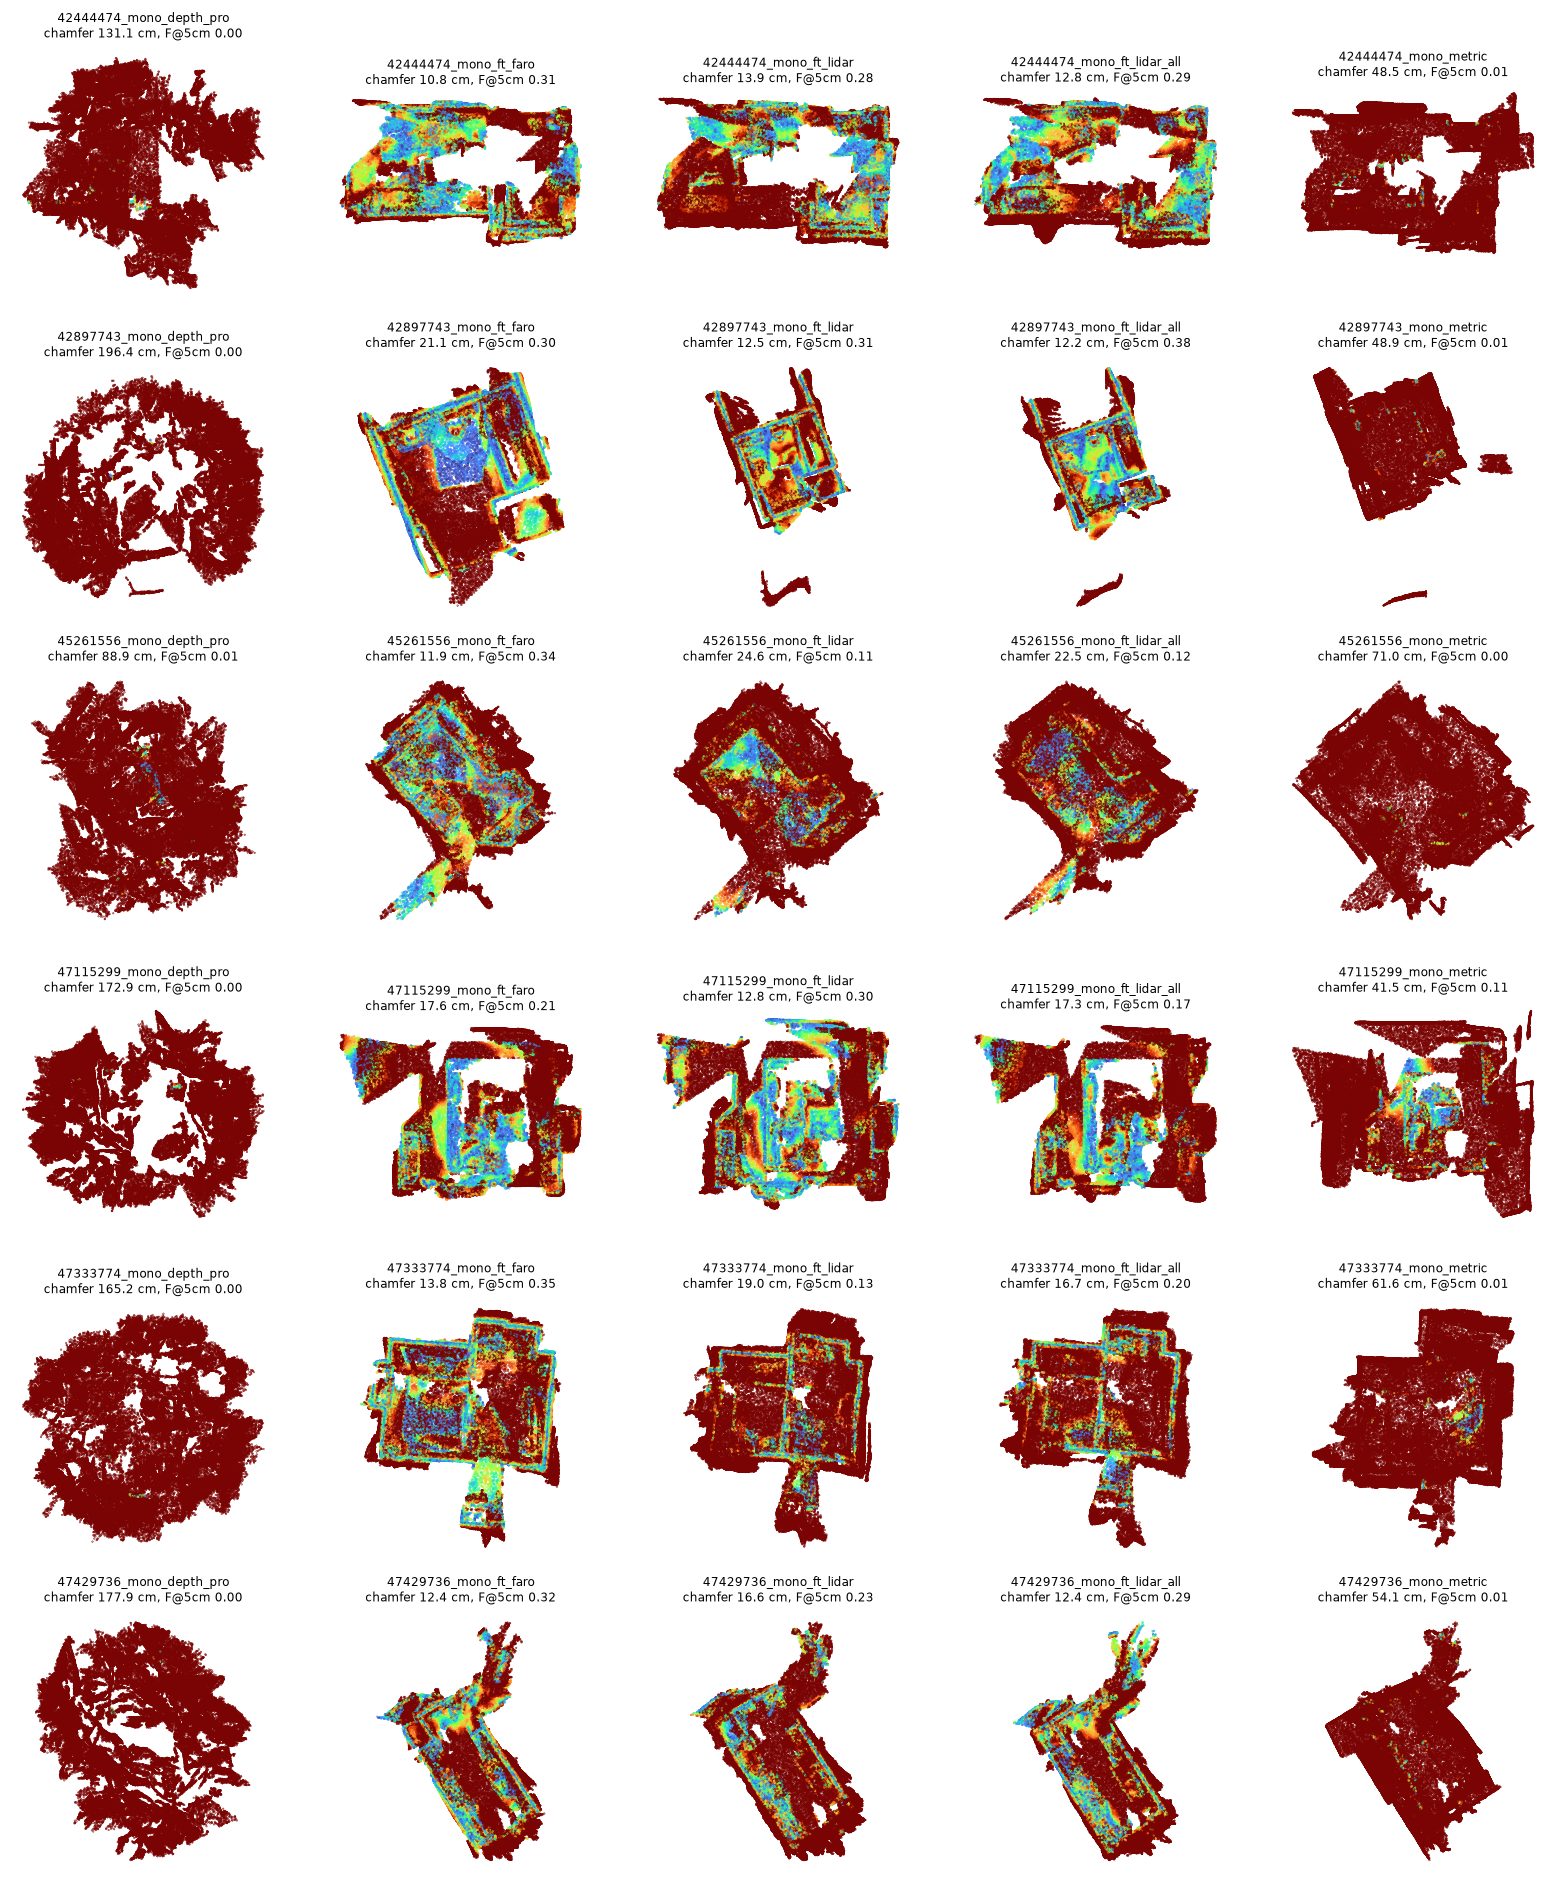
\includegraphics[width=\gridw]{exp6_finetune_topdown_grid}};
% cover the per-panel titles of the generated image (run names, per-panel Chamfer)
\foreach \x/\y in {45/12, 366/59, 684/57, 1001/56, 1318/52, 45/331, 366/322, 684/322, 1001/322, 1318/323,
                   45/635, 366/635, 684/635, 1001/635, 1318/636, 45/966, 366/985, 684/975, 1001/983, 1318/967,
                   45/1268, 366/1262, 684/1262, 1001/1262, 1318/1263, 45/1576, 366/1576, 684/1576, 1001/1576, 1318/1577}
  \fill[white] (\x-6,\y-4) rectangle ++(208,36);
\foreach \x/\t in {143/Depth Pro, 460/\ftfaro, 777/\ftlidar, 1095/\ftmain, 1412/pretrained}
  \node[anchor=south] at (\x,4) {\t};
\foreach \y/\t in {150/42444474, 465/42897743, 790/45261556, 1110/47115299, 1420/47333774, 1730/47429736}
  \node[rotate=90, anchor=south] at (-4,\y) {\t};
\end{tikzpicture}
\caption{Exp.~6 seen from above: every point of the reconstructed mesh coloured by its distance to the Faro mesh, from
dark blue (\SI{0}{cm}) through green and yellow to dark red (\SI{10}{cm} or more). Rows are rooms, by scan ID;
columns are models.}
\label{fig:exp6}
\end{figure}

\subsection{Place among the run-time depth sources (objective 3)}\label{sec:exp1}
\begin{table}[t]
\centering\small
\caption{Exp.~1, six test rooms: only the depth source and the scale alignment change (\ftmain{} from Exp.~6).
Recall at 10, 5 and \SI{2}{cm}: room overview, furniture placement, renovation measurement; for rows usable at run
time, \checkmark{} served ($\geq0.9$), $\sim$ partly (0.75--0.9), $\times$ not ($<0.75$).}
\label{tab:exp1}
\setlength{\tabcolsep}{3.5pt}
\begin{adjustbox}{max width=\columnwidth}
\begin{tabular}{@{}llrrrlll@{}}
\toprule
 & & & & & \multicolumn{3}{c}{Recall at} \\ \cmidrule(l){6-8}
Source & Alignment & Chamfer & F@5 & AbsRel & \SI{10}{cm} & \SI{5}{cm} & \SI{2}{cm} \\
\midrule
Faro & none & $\rsGTCM \pm \rsGTSD$ & \rsGTF & 0 & \rsGTRten & \rsGTRfive & \rsGTRtwo \\
iPad LiDAR & none & $\rsLIDARCM \pm \rsLIDARSD$ & \rsLIDARF & \rsLIDARABSREL & \checkmark~\rsLIDARRten & \checkmark~\rsLIDARRfive & $\times$~\rsLIDARRtwo \\
DA-v2 Large & per-frame oracle & $\rsORACLECM \pm \rsORACLESD$ & \rsORACLEF & \rsORACLEABSREL & \rsORACLERten & \rsORACLERfive & \rsORACLERtwo \\
DA-v2 Large & sparse points & $\rsSPARSECM \pm \rsSPARSESD$ & \rsSPARSEF & \rsSPARSEABSREL & \checkmark~\rsSPARSERten & $\sim$~\rsSPARSERfive & $\times$~\rsSPARSERtwo \\
DA-v2 Large & once per room & $\rsSCENECM \pm \rsSCENESD$ & \rsSCENEF & \rsSCENEABSREL & $\times$~\rsSCENERten & $\times$~\rsSCENERfive & $\times$~\rsSCENERtwo \\
DA-v2 Metric-Indoor & none & $\rsMETRICCM \pm \rsMETRICSD$ & \rsMETRICF & \rsMETRICABSREL & $\times$~\rsMETRICRten & $\times$~\rsMETRICRfive & $\times$~\rsMETRICRtwo \\
\textbf{\ftmain{}} & none & $\rsFTLIDARALLCM \pm \rsFTLIDARALLSD$ & \rsFTLIDARALLF & \rsFTLIDARALLABSREL & $\times$~\rsFTLIDARALLRten & $\times$~\rsFTLIDARALLRfive & $\times$~\rsFTLIDARALLRtwo \\
\bottomrule
\end{tabular}
\end{adjustbox}
\end{table}

Through the same pipeline (Table~\ref{tab:exp1}), Faro depth itself gave \SI{\rsGTCM}{cm}. iPad LiDAR gave
\SI{\rsLIDARCM}{cm}, \SI{\rsLIDARGAPGTCM \pm \rsLIDARGAPGTSD}{cm} above Faro per room and above it in every room; its
recall at \SI{2}{cm} was \rsLIDARRtwo{}, against \rsGTRtwo{} for Faro. DA-v2 Large with the per-frame oracle gave
\SI{\rsORACLECM}{cm}, \SI{\rsORACLEGAPLIDARCM \pm \rsORACLEGAPLIDARSD}{cm} above LiDAR per room; aligned on sparse points
it gave \SI{\rsSPARSECM}{cm}, and aligned once per room \SI{\rsSCENECM}{cm}, between \rsSCENEc{} and
\SI{\rsSCENEb}{cm} in every room. The pretrained DA-v2 Metric-Indoor gave \SI{\rsMETRICCM}{cm}; in room 45261556 it had
its highest Chamfer distance (\SI{\rsMETRICf}{cm}) while the per-frame oracle had its second lowest there
(\SI{\rsORACLEf}{cm}; Table~\ref{tab:perroom}). By the thresholds of Section~\ref{sec:metrics}, iPad LiDAR served the
overview and furniture placement, sparse points served the overview and partly served furniture placement, and no
row, \ftmain{} included, served renovation measurement.

\begin{table}[t]
\centering\small
\caption{Per test room, in the order of Table~\ref{tab:scenes} (first four digits of the scan ID). DA-v2 L: DA-v2
Large.}
\label{tab:perroom}
\begin{adjustbox}{max width=\columnwidth}
\begin{tabular}{@{}lrrrrrrr@{}}
\toprule
 & 4244 & 4733 & 4711 & 4289 & 4742 & 4526 & mean \\
\midrule
\multicolumn{8}{@{}l}{\emph{Chamfer distance (cm)}} \\
Faro & \rsGTa & \rsGTb & \rsGTc & \rsGTd & \rsGTe & \rsGTf & \rsGTCM \\
iPad LiDAR & \rsLIDARa & \rsLIDARb & \rsLIDARc & \rsLIDARd & \rsLIDARe & \rsLIDARf & \rsLIDARCM \\
DA-v2 L, per-frame oracle & \rsORACLEa & \rsORACLEb & \rsORACLEc & \rsORACLEd & \rsORACLEe & \rsORACLEf & \rsORACLECM \\
DA-v2 L, sparse points & \rsSPARSEa & \rsSPARSEb & \rsSPARSEc & \rsSPARSEd & \rsSPARSEe & \rsSPARSEf & \rsSPARSECM \\
DA-v2 L, once per room & \rsSCENEa & \rsSCENEb & \rsSCENEc & \rsSCENEd & \rsSCENEe & \rsSCENEf & \rsSCENECM \\
pretrained DA-v2 Metric & \rsMETRICa & \rsMETRICb & \rsMETRICc & \rsMETRICd & \rsMETRICe & \rsMETRICf & \rsMETRICCM \\
Depth Pro & \rsDEPTHPROa & \rsDEPTHPROb & \rsDEPTHPROc & \rsDEPTHPROd & \rsDEPTHPROe & \rsDEPTHPROf & \rsDEPTHPROCM \\
\ftfaro & \rsFTFAROa & \rsFTFAROb & \rsFTFAROc & \rsFTFAROd & \rsFTFAROe & \rsFTFAROf & \rsFTFAROCM \\
\ftlidar & \rsFTLIDARa & \rsFTLIDARb & \rsFTLIDARc & \rsFTLIDARd & \rsFTLIDARe & \rsFTLIDARf & \rsFTLIDARCM \\
\textbf{\ftmain{}} & \rsFTLIDARALLa & \rsFTLIDARALLb & \rsFTLIDARALLc & \rsFTLIDARALLd & \rsFTLIDARALLe & \rsFTLIDARALLf & \rsFTLIDARALLCM \\
\midrule
\multicolumn{8}{@{}l}{\emph{AbsRel}} \\
pretrained DA-v2 Metric & \rsMETRICARa & \rsMETRICARb & \rsMETRICARc & \rsMETRICARd & \rsMETRICARe & \rsMETRICARf & \rsMETRICSIXABSREL \\
\textbf{\ftmain{}} & \rsFTALLARa & \rsFTALLARb & \rsFTALLARc & \rsFTALLARd & \rsFTALLARe & \rsFTALLARf & \rsFTLIDARALLABSREL \\
\bottomrule
\end{tabular}
\end{adjustbox}
\end{table}

\subsection{Per-frame scale (objective 4)}\label{sec:scale}
\begin{table}[t]
\centering\small
\caption{Per-frame scale of the pretrained model and \ftmain{}, every fifth frame of the six test rooms (471 frames).
Ratio: Faro depth over predicted depth, median over the pixels of a frame.}
\label{tab:scale}
\begin{adjustbox}{max width=\columnwidth}
\begin{tabular}{@{}lrr@{}}
\toprule
 & Pretrained & \textbf{\ftmain{}} \\
\midrule
ratio, median over the frames of a room (range over rooms) & 0.69--0.85 & \textbf{0.93--1.21} \\
ratio, 95th over 5th percentile within a room (mean) & 1.55 & 1.52 \\
AbsRel, no help & 0.381 & \textbf{0.134} \\
AbsRel, one scale and offset per room from 10 frames & 0.127 & 0.117 \\
AbsRel, the right scale on every frame & 0.045 & 0.051 \\
AbsRel, per-frame oracle scale and offset & 0.035 & 0.042 \\
\bottomrule
\end{tabular}
\end{adjustbox}
\end{table}

For the pretrained model, the median ratio of Faro to predicted depth was 0.69 to 0.85 in the six rooms, so its
predicted depth was 1.18 to 1.45 times the Faro depth; for \ftmain{} the ratio was 0.93 to 1.21
(Table~\ref{tab:scale}). Within a room, the 95th percentile of the ratio was on average 1.55 times its 5th percentile
for the pretrained model and 1.52 times for \ftmain{}; in room 47115299 the pretrained model's ratio ranged from 0.43 to
1.35. With no help, \ftmain{} had AbsRel 0.134, against 0.127 for the pretrained model with one scale and offset per
room fitted on Faro depth. With the right scale on every frame, AbsRel fell to 0.045 for the pretrained model, 97\,\%
of the way from no help to the oracle, and to 0.051 for \ftmain{}.

\begin{figure}[t]
\centering
\begin{tikzpicture}
\begin{axis}[width=0.95\columnwidth, height=0.55\columnwidth, xmode=log, ymode=log, xmin=0.3, xmax=6, ymin=0.2,
  ymax=5, xtick={0.5,1,2,4}, xticklabels={0.5,1,2,4}, ytick={0.25,0.5,1,2,4}, yticklabels={0.25,0.5,1,2,4},
  tick label style={font=\scriptsize}, label style={font=\footnotesize}, grid=major, grid style={black!8},
  xlabel={median Faro depth of the frame (m)}, ylabel={per-frame scale / per-room scale}]
\addplot[black!55, dashed, domain=0.3:6, samples=2] {1};
\addplot[only marks, mark=*, mark size=0.8pt, blue!70!black, fill opacity=0.5, draw opacity=0.5]
  table[x=depth, y=ratio] {../figures/data/scale_vs_depth.dat};
\end{axis}
\end{tikzpicture}
\caption{Relative model DA-v2 Large, every fifth frame of the six test rooms: the per-frame oracle scale divided by
the once-per-room scale, against the median Faro depth of the frame (469 frames; two frames whose fit gave no positive
scale are left out). Pearson correlation of the logarithms: $-0.37$.}
\label{fig:scalevsdepth}
\end{figure}

For the relative model DA-v2 Large, the per-frame oracle scale varied within a room by a factor of 2.6 to 4.9 between
its 5th and 95th percentiles. Its correlation with the frame's time in the scan ranged from $-0.40$ to $+0.30$, positive
in three rooms and negative in three; its correlation with the frame's median Faro depth ranged from $-0.75$ to
$-0.27$, negative in all six (Fig.~\ref{fig:scalevsdepth}).

\subsection{Sensitivity of the pipeline (Exp.~2--5)}\label{sec:secondary}
\begin{table}[t]
\centering\small
\caption{Sensitivity experiments on the six test rooms; one setting changes, everything else as in Section~\ref{sec:method}.}
\label{tab:secondary}
\footnotesize
\begin{tabularx}{\columnwidth}{@{}l>{\raggedright\arraybackslash}X@{}}
\toprule
Exp. & Result \\
\midrule
2 voxel size & Faro depth; 2 / 4 / \SI{8}{cm}: Chamfer 1.2 / 2.1 / \SI{2.8}{cm}; fusion at most \SI{2}{s} per room at every size \\
3 frame stride & Faro depth; every 1st / 5th / 10th frame (4 / 0.8 / 0.4 per second): accuracy \rsSTRGTONEACC{} / \rsSTRGTFIVEACC{} / \SI{\rsSTRGTTENACC}{cm},
completeness \rsSTRGTONECOMP{} / \rsSTRGTFIVECOMP{} / \SI{\rsSTRGTTENCOMP}{cm}, \fscore{} \rsSTRGTONEF{} / \rsSTRGTFIVEF{} / \rsSTRGTTENF{} \\
4 model size & per-frame oracle; DA-v2 Large (335\,M parameters) / Small (25\,M) / MiDaS small (21\,M): Chamfer
\rsDALARGECM{} / \rsDASMALLCM{} / \SI{\rsMIDASCM}{cm}; \rsDALARGESCAN{} / \rsDASMALLSCAN{} / \SI{\rsMIDASSCAN}{s} per room \\
5 LiDAR confidence & Chamfer \SI{3.04}{cm} with every pixel, \SI{\rsCONFONECM}{cm} without low-confidence pixels,
\SI{\rsCONFTWOCM}{cm} with high-confidence pixels only (completeness 3.85 $\rightarrow$ \SI{\rsCONFTWOCOMP}{cm}),
\rsWOTFCM{} and \SI{\rsWZOTCM}{cm} with pixels weighted by confidence \\
\bottomrule
\end{tabularx}
\end{table}

Table~\ref{tab:secondary} lists the sensitivity experiments. DA-v2 Small gave a Chamfer distance \SI{1.0}{cm} higher
than DA-v2 Large and was 6.4 times faster per room; at four frames per second, processing took 3.6 times the length of
the video with DA-v2 Large and 0.6 times with DA-v2 Small, of which fusion was less than 3\,\%.

\section{Discussion and Conclusion}\label{sec:discussion}
% Thai version: 05_discussion_th.tex (main_short_th.tex); keep the two in step.
% Replaces the former 06_discussion.tex + 08_limitations.tex + 09_conclusion.tex of the short version.
% Every number here is reported in Section IV; this chapter interprets, relates to prior work and qualifies.

This section relates the results to prior work, interprets the error that remains, draws implications, states the
limitations and future work, and concludes objective by objective.

\subsection{Relation to prior work}\label{sec:prior}
\mbox{DA-v2} Metric-Indoor learned metres from the rendered rooms of Hypersim~\cite{da2,hypersim} and placed every real
test room 1.18 to 1.45 times too far. ZoeDepth~\cite{zoedepth} and \mbox{DA-v2} adapt their metric heads to a target
domain by fine-tuning on labelled data; our result shows that the same remedy works with the target device's own LiDAR
as the labels. As the DINOv2 authors did for depth~\cite{dinov2}, we trained only the decoder on the frozen encoder,
and the shape of the prediction barely changed (per-frame oracle AbsRel 0.035 against 0.042), which fits the view that
the encoder's features transfer~\cite{yosinski} and the head mainly learned the scale.

Sensor depth has long served as a training label, from Kinect indoors to laser scanners on
cars~\cite{nyuv2,kitti,eigen14}. The roughly \SI{1}{cm} that phone LiDAR adds to the Faro depth in our pipeline agrees
with the centimetre-level accuracy reported against surveying methods~\cite{luetzenburg,spreafico}, and its error as a
label (AbsRel \rsLIDARABSREL{}) is an order of magnitude below the error left in the fine-tuned model
(\rsFTLIDARALLABSREL{}), which may explain why a laser teacher gave no measurable gain. Prompt Depth
Anything~\cite{promptda} and the upsampling task of ARKitScenes~\cite{arkitscenes} use the LiDAR at run time; our model
needs only a colour image, at a large price (\SI{\rsFTLIDARALLCM}{cm} against \SI{\rsLIDARCM}{cm}).

Camera-aware models~\cite{metric3d,unidepth,depthpro} treat the unknown focal length as the main obstacle to metric
depth. For Depth Pro on these $640\times480$ indoor frames, the true focal length did not make it usable, and its error
without scale stayed several times that of \mbox{DA-v2} Metric-Indoor; we did not test Metric3D or UniDepth, so this
does not extend to the approach in general. Per-image benchmarks cannot show whether the scale stays the same across
the frames of a scan (Section~\ref{sec:related}); we found that it does not, for relative and metric models alike.
Video Depth Anything~\cite{videoda} targets such consistency across video frames, and sparse metric points, used as in
CNN-SLAM and MonoSDF~\cite{cnnslam,monosdf}, came within \SI{\rsSPARSEGAP}{cm} of the per-frame oracle in their
upper-bound form. Learned reconstruction systems~\cite{atlas,neuralrecon,simplerecon} use several frames per prediction
and other data, so our numbers are not comparable with theirs.

\subsection{Why a scale error remains}\label{sec:whyft}
Fine-tuning learned the domain's multiplier: \ftmain{} without calibration (AbsRel 0.134) is on a par with the
pretrained model given one scale and offset per room fitted on ground truth (0.127), so what a one-off calibration
provides has moved into the weights of the head. The swing from frame to frame did not shrink (1.52 against 1.55). A
likely reason follows from the pinhole model (Section~\ref{sec:related}): views such as a close-up of a table top or a
blank wall look alike at different distances and give no cue to absolute size, so the model falls back on a typical
indoor distance; the negative correlation between the needed scale and the depth of the view, found in every room, fits
this reading. If it is right, more or better labels will not remove the swing, and metric data at run time will be
needed. TSDF fusion~\cite{curless96} then averages the same surface placed at several distances into a thicker, blurred
surface, consistent with a moderate per-frame error becoming \SI{\rsFTLIDARALLCM}{cm} in Chamfer distance.

\subsection{Implications for practice}\label{sec:business}
For an app on a device without LiDAR, the results suggest an order of work: per-frame metric scale first (within
\SI{\rsSPARSEGAP}{cm} of the per-frame oracle, against \SI{\rsSCENECM}{cm} with one calibration per room, an upper bound
because the points came from LiDAR, not from VIO), then a fine-tuned model, which removes the domain bias with nothing at
run time, and model size last (\mbox{DA-v2} Small was \SI{1.0}{cm} worse than Large under the per-frame oracle and 6.4
times faster). The labels can be collected from Pro devices during normal use, since ARKit delivers colour, LiDAR depth
and pose together. At 3.6 times the video length on a laptop, the pipeline as tested runs offline.

\subsection{Limitations}\label{sec:limitations}
The evaluation is small: six test rooms in 3D, one used during development, and 26 rooms per frame, all homes captured
with one iPad model; offices, empty rooms, low light and other phone cameras are absent, and the bathroom with a mirror
was the hardest room for every source with the right scale (Table~\ref{tab:perroom}). With six rooms the Wilcoxon test
detects only a difference present in every room, so the teacher comparison cannot rule out differences of the size seen
in the means, one to two centimetres. The main comparison was fixed after the six test rooms had been evaluated; the
\rsVN{} rooms of Exp.~7 were added afterwards so that the conclusion also rests on rooms that decided nothing. The
reference shares the ARKit poses of every row, so a real phone system would add pose drift, and completeness is relative
to what Faro saw. Only the head of one model was fine-tuned, with one recipe, and \ftfaro{} and \ftlidar{} differ in
the number of views as well as the labels. Checkpoints were chosen with Faro depth, also for the LiDAR-taught models, on
three rooms; \ftmain{} became the main model because it was best there and its labels need no laser scanner, but that
ranking did not reproduce on the test rooms, and its validation AbsRel changed by up to 0.1 between checkpoints 500
steps apart. The once-per-room and sparse-point
alignments are upper bounds, calibrated on ground truth and on clean LiDAR samples. Depth Pro was run through one
implementation, and its focal-length check covered five frames of one room. The thresholds that link recall to use
cases are our illustration, not an industry standard, and times are unoptimised and meaningful only as ratios.

\subsection{Future work}\label{sec:future}
In order of expected impact, future work should (1)~combine \ftmain{} with per-frame metric points from the device's
tracker, for which Section~\ref{sec:scale} gives AbsRel 0.051 with the right scale on every frame; (2)~choose
checkpoints with LiDAR depth, so that no step needs a laser scanner, and compare teachers on identical frames and more
test rooms; (3)~train and evaluate on more phone cameras, including Android; (4)~evaluate with real ARKit or ARCore
feature points and a reference captured by the app itself; and (5)~test fine-tuning more of the network, and video
models that keep the scale consistent across frames~\cite{videoda}.

\subsection{Conclusion}\label{sec:conclusion}
We asked whether fine-tuning a metric monocular depth model with a phone's own LiDAR makes it more accurate than its
pretrained self against a laser scanner. For objective~(1) it did, on the rooms tested and by the criterion of the
Introduction: \ftmain{} lowered the Chamfer distance from \rsMETRICCM{} to \SI{\rsFTLIDARALLCM}{cm} in all six test rooms
and AbsRel from \rsVMETRICABSREL{} to \rsVFTALLABSREL{} in \rsVWINS{} of \rsVN{} further rooms, with no calibration or
sensor at run time and with weights learned from LiDAR alone, although \wone{} improved in only five of the six test
rooms. For objective~(2), laser labels were not measurably better than LiDAR labels, nor 24 rooms better than 10, within
the limited power of six rooms, and the true focal length did not make Depth Pro competitive. For objective~(3), the
model lies between a relative model calibrated once per room and one aligned on sparse points in every frame, serves
none of the three use cases, and is no substitute for iPad LiDAR (\SI{\rsLIDARCM}{cm}). For objective~(4), its remaining
error is a scale that varies with the view rather than drifting with time, whose bias fine-tuning removed but whose
spread it did not. Per-frame metric points from the device's tracker are the most promising next step; their
combination with the fine-tuned model remains to be tested.


\bibliographystyle{IEEEtran}
\bibliography{refs}

\end{document}
